\scanpage{252}
\diagram{\begin{tikzcd}
\mathcal N=\operatorname{Mod}(k)\arrow[r,"i"]&
\mathcal M_0=\mathcal M^+\arrow[l,bend left,"{\deleted{\unsure{\kappa}}p}"]
\end{tikzcd}}
\deleted{\(\unsure{\mathcal N\longrightarrow\mathcal M_N}\)}
\(\boxed{i,p,\unsure{r|S}}\)
\[
i(N)=N\otimes_kS,\qquad\unsure{\kappa}(M)=M_0.
\]
\[
\tau_{N,0}\circ i:\mathcal N\longrightarrow\mathcal M_N
\]
a comme adjoint à droite
\[
\kappa\circ\rho_{0N}=\kappa\circ\tau_0\circ\rho_N=\kappa\circ\rho_N.
\]
\margin{\deleted{qui a comme adjoint à gauche}}
\uline{Conditions équivalentes}

 a) \(i_N=\tau_{N,0}\circ i\) est pl. fidèle

 b) \(\forall\unsure{P}\in\operatorname{Mod}k,\quad
 \unsure{P}\overset\sim\longrightarrow(\rho_Ni_N(\unsure{P}))_0\)
\[
\left[\begin{aligned}
&=(\rho_N\tau_N(\unsure{P}\otimes_k S))_0\\
&=(\rho_N(P\otimes_k\tau_NS))_0
\end{aligned}\right]
\]
 c) \(\kappa\circ\rho_N\) est un foncteur localisation.

\figure{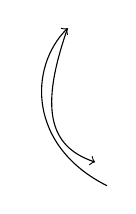
\begin{tikzpicture}[scale=.5]
\draw[->] (1,0) .. controls (-1,1) and (-1,3) .. (0,4);
\draw[->] (0,4) .. controls (-.7,2) and (-.5,1) .. (.7,.6);
\end{tikzpicture}}
\deleted{\diagram{\begin{array}{ccc}
\mathcal M_0&\unsure{\mathcal M_1}&\unsure{\mathcal M_N}\\
\downarrow&&\\
\unsure{P_k}&&
\end{array}}}
\deleted{\(\unsure{\operatorname{Hom}_k(P,Q)}\)}

\uline{Conditions équivalentes}

 a') \(\deleted{\unsure{\forall P\in\operatorname{Mod}k}}
 \operatorname{Imess}i\subset\operatorname{Imess}\rho_{0N}\)

 b') \(\forall P\in\operatorname{Mod}k,\quad
 iP\overset\sim\longrightarrow\rho_{0N}\tau_{N,0}\circ i(P)
 =\rho_{0N}i_N(P)\)

 \unsure{b') bis} \(\forall P\in\operatorname{Mod}k,\quad
 i(P)\overset\sim\longrightarrow\rho_{0N}i_N(P)\) est un isom en degrés
 \(0\leq\alpha\leq N-1\).

 c') \(\inserted{\forall P\in\operatorname{Mod}k,}\quad
 \forall\ 0\leq\alpha\leq N-1,\quad
 \deleted{\unsure{\tau_{N-\alpha,0}S\longrightarrow0}}\)
\diagram{\begin{tikzcd}
P\otimes_k S_\alpha\arrow[r,"\sim"]&
\operatorname{Hom}^\alpha(\tau_{N-\alpha}S,\deleted{\unsure{P}}P\otimes_kS)\\
\bigl[\operatorname{Hom}^\alpha(S,P\otimes_kS)\arrow[u,"\simeq"]
\arrow[ur,dashed,"\text{restriction}"']&\bigr]
\end{tikzcd}}
\[
\operatorname{Hom}^\alpha(S/\tau_{N-\alpha}S,P\otimes_kS)=0.
\]
\margin{251}
